% Created 2020-05-17 Sun 23:14
% Intended LaTeX compiler: pdflatex
\documentclass[presentation]{beamer}
\usepackage[utf8]{inputenc}
\usepackage[T1]{fontenc}
\usepackage{graphicx}
\usepackage{grffile}
\usepackage{longtable}
\usepackage{wrapfig}
\usepackage{rotating}
\usepackage[normalem]{ulem}
\usepackage{amsmath}
\usepackage{textcomp}
\usepackage{amssymb}
\usepackage{capt-of}
\usepackage{hyperref}
\usetheme{default}
\date{}
\title{SEM: A Simulation Execution Manager for ns-3}
\hypersetup{
 pdfauthor={},
 pdftitle={SEM: A Simulation Execution Manager for ns-3},
 pdfkeywords={},
 pdfsubject={},
 pdfcreator={Emacs 26.3 (Org mode 9.3.6)},
 pdflang={English}}
\begin{document}

\maketitle


\begin{frame}[label={sec:org430bc56},fragile]{Setup!}
 This lesson requires some setup. We will download a new copy of ns-3, and use
that one for the rest of this lab.

\begin{block}{Open up a terminal!}
\begin{verbatim}
cd
git clone --recursive https://github.com/DvdMgr/sem-lab
cd sem-lab
ls -l
\end{verbatim}
\end{block}
\end{frame}

\begin{frame}[label={sec:orgde3c64d},fragile]{What is in this folder?}
 \begin{block}{This is what you should see in the sem-lab folder}
\begin{description}
\item[{\texttt{ns-3}}] Our new ns-3 installation folder
\item[{\texttt{params}}] Ignore this for now!
\item[{\texttt{Slides}}] Folder containing this lesson's slides
\item[{\texttt{wifi-plot.m}}] Octave script to plot the results of our simulations
\item[{\texttt{wifi-sem.cc}}] The ns-3 simulation script we will run
\end{description}
\end{block}

\begin{block}{Let's compile ns-3}
\begin{verbatim}
cd ns-3
./waf configure build
\end{verbatim}
\end{block}
\end{frame}

\begin{frame}[label={sec:org60479b9},fragile]{Summary of what \texttt{wifi-sem.cc} does}
 \begin{itemize}
\item Creates a WiFi network
\item Provides a set of command line arguments we can use
\begin{itemize}
\item Distance from AP
\item Number of devices
\item MCS
\item Using Request To Send (RTS)
\item Using Short Guard Interval (SGI)
\item Randomness of channel
\end{itemize}
\item Prints the throughput of the network
\end{itemize}
\end{frame}

\begin{frame}[label={sec:org2a38775},fragile]{Playing around with the wifi-sem script}
 Try some arguments!

\begin{verbatim}
./waf --run "wifi-sem --useRts=False"
./waf --run "wifi-sem --useRts=True"
./waf --run "wifi-sem --mcs=3 --RngRun=1"
./waf --run "wifi-sem --mcs=3 --RngRun=2"
\end{verbatim}
\end{frame}

\begin{frame}[label={sec:orga53e0e1},fragile]{What is SEM?}
 SEM is a Python library and program that allows you to:
\begin{itemize}
\item Run multiple simulations in parallel from the command line
\item Export results to various formats (folders, MATLAB)
\item Perform both simulations and analysis from the same Python script
\end{itemize}

SEM is already installed in your system:
\begin{verbatim}
sem --help
\end{verbatim}
\end{frame}

\begin{frame}[label={sec:org64b9214},fragile]{Running the program with SEM}
 Try it! \emph{Make sure to be in the \texttt{sem-lab} folder for this (\texttt{cd ..}).}

The \texttt{sem run} command can be used to run simulations:

\begin{verbatim}
sem run --help
\end{verbatim}

Use [Value1, Value2, \ldots{}] to specify multiple values.
\end{frame}

\begin{frame}[label={sec:org9e35f3a},fragile]{Viewing results}
 The \texttt{sem view} command can be used to view results of previously run
simulations:

\begin{verbatim}
sem view --help
\end{verbatim}
\end{frame}

\begin{frame}[label={sec:org0477560},fragile]{Exporting results}
 The export command can be used to export results:
\begin{verbatim}
sem export --help
\end{verbatim}

Let's export results to a nested folder structure:
\begin{verbatim}
sem export results-directory
\end{verbatim}
\end{frame}

\begin{frame}[label={sec:org0cabe5d},fragile]{Exporting results to MATLAB and plotting}
 Clean up your results folder with the \texttt{rm -r res} command.

Run simulations using a pre-specified parameter space:

\begin{verbatim}
sem run --parameters params
\end{verbatim}

Export results to MATLAB data structure:

\begin{verbatim}
sem export results.mat --results-dir res
\end{verbatim}

Run the MATLAB script to plot results:

\begin{verbatim}
octave --persist wifiplot.m
\end{verbatim}
\end{frame}

\begin{frame}[label={sec:orga3cccc6},fragile]{Exercise}
 \alert{Plot the throughput for increasing mcs and for every setting of SGI and RTS
at a fixed distance.}

\begin{itemize}
\item Reset your results directory
\begin{verbatim}
rm -r res
\end{verbatim}
\item Make sure you run all the simulations you need
\begin{itemize}
\item What values for MCS, SGI and RTS?
\end{itemize}
\item Export results
\item Modify \texttt{wifiplot.m} to create the new plot
\end{itemize}

\begin{center}
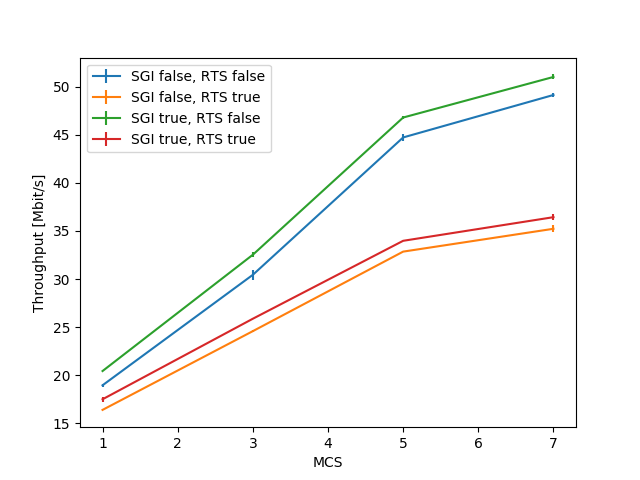
\includegraphics[width=0.5\textwidth]{mcssgirts.png}
\end{center}
\end{frame}
\end{document}